\section{Theoretical Background}
The Superconducte was discovered in 1911 by Heike Kamerlingh Onnes, while
investigating the temperature dependence of electrical resistance.
He noticed the disappereance of resistance of mercury below 4.2 K and
after this discovery more materials were found to have this superconducting property.
\ldots






\subsection{magnetic field}
Following we can straightaway calculate the magnetic field using
Biot-Savart law (see figure~\ref{fig:magnetic_field}):
We start with the law of Biot-Savart of a electric flow $I$ along the path $C$ which generates
a magnetic field $B$ at position $r$:
\begin{equation}
    \vec{B} = \frac{\mu_0}{4\pi} \int_{C} \frac{I d\vec{l} \times \vec{r}}{|\vec{r}|^3} 
\end{equation}
which can be rewritten, if we use the absolute value instead of vectors and the Radius $r$ of the
coil with the horizontal position $x$:
\begin{equation}
    dB = \frac{\mu_0}{4\pi} \frac{N \cdot I dl}{(r^2 + z^2)} 
\end{equation}

We only need the fraction of the z-direction. Let now $\theta$ be the angle betwen the $y,z$ 
direction and the $x-$axis using $\sqrt{{r}^2 + x^2} \cos(\theta) = {r}$:
\begin{align}
     dB_z &= dB \cos\theta = dB \left (\frac{{r}}{\sqrt{{r}^2 + z^2}} \right) = 
    \frac{\mu_0}{4\pi} \frac{N\cdot I  \cdot {r} \cdot dl}{\sqrt{\left ({r}^2 + z^2 \right )^3}} \\
\Rightarrow B_z &= \frac{\mu_0}{4\pi} \frac{N\cdot I  \cdot {r}}{\sqrt{\left ({r}^2 + z^2 \right )^3}} \int_C dl 
  = \frac{\mu_0}{4\pi} \frac{N\cdot I  \cdot {r}}{\sqrt{\left ({r}^2 + z^2 \right )^3}} \left (2\pi {r} \right )
  =  \frac{\mu_0}{2} \frac{N\cdot I  \cdot {r}^2}{\sqrt{\left ({r}^2 + z^2 \right )^3}} \\
  &\approx \frac{\mu_0\cdot N \cdot I \cdot r^2}{2z^3}.
\end{align}
Where in the last approximation we used the fact that for large $z$, the
radius is neglectable.
\begin{figure}[htpb]
    \centering
    \includegraphics[width=0.4\linewidth]{figures/magnetic_field}
    \caption{Sketch for the derivation of the magnetic field using Biot-Savart law.}
    \label{fig:magnetic_field}
\end{figure}

\section{Technical details}
In this section wo want to go into the devices which will be used during the
conduction of the experiment.
\subsection{The SQUID (Superconducting Quantum Interference Device} represents a magnetic field
detector of great precision, using the already stated superconducting flux quantization and
the josephson effect. We will use a RF-Squid, which operates with one single josephson junction
\footnote{The first squid to be invented was a DC-Squid, having two josephson junctions in parallel. In 1962
the josephson effect was postulated by Brian David Josephson, and already 1963 the first josephson junction
was implemented by Philip Anderson. One year later, in 1964 the DC SQUID was invented by Robert Jaklevic, John J. Lambe
and James Mercereau.} through an AC current, where the Josephson junction in this case is a thin isolation.
\subsection{Lock-in method}
\paragraph{In order to supress}
noise and frequencies from other processes, we use
a frequently used method called ``lock-in amplification''. Depending on the
setup it is possible to reduce the noise by a factor $10^6$. The method
is based on the orthogonality relation of sinusoidal functions (which
can be seen easily differentiating the left with respect to $x$):
\begin{equation}
    \int \sin(a x) \sin(b x) dx =\frac{ b \sin(a x) \cos(b x)-a \cos(a x)
            \sin(b x)}{a^2-b^2}
\end{equation}
If we let the integration go from $\infty$ to $-\infty$ we end up with:
\begin{equation}
    (a,b) := \int_{-\infty}^{\infty} \sin(a x) \sin(b x) dx = \delta(a - b)
\end{equation}
Which stems from the sinusoidal functions forming a complete basis with
the integral as inner product.\\
Since we will not manipulate the parameters of the lock-in method in this
experiment, we will not go into the technical details, which
will also not be object of the analysis.
